\documentclass{article}
\usepackage[utf8]{inputenc}

\title{Assignment 6(b) - The Laplace Transform}
\author{Jahnavi Pragada}
\date{\today}


\usepackage{natbib}
\usepackage{graphicx}
\usepackage{amsmath}
\usepackage{listings}

\begin{document}

\maketitle

\section*{Introduction}
In this assignment, we will look at how to analyze “Linear Time-invariant Systems” using the scipy.signal library in Python .All the problems are in continuous time and use Laplace Transforms. We considered systems: A forced oscillatory system, A coupled system of Differential Equations and an RLC low pass filter  


\section*{Question 1,2}
We first consider the forced oscillatory system(with 0 initial conditions):
\begin{equation}
    \ddot x + 2.25x = f(t)
\end{equation}
We solve for $X(s)$ using the following equation, derived from the above equation.
\begin{equation}
    X(s) = \frac{F(s)}{s^2+2.25}
\end{equation}
We then use the impulse response of $X(s)$ to get its inverse Laplace transform.We found for two different decay constants 0.5,0.05



\begin{verbatim}
def func(decay, w):
    Xn = np.poly1d([1, decay])
    Xd = np.polymul([1, 0, 2.25], [1, 2*decay, (w**2 + decay**2)])
    Xs = sp.lti(Xn, Xd)
    t, x = sp.impulse(Xs, None, np.linspace(0, 50, 500))
    return Xs, t, x
    
X, t1, x1 = func(0.5, 1.5)
X, t2, x2 = func(0.05, 1.5)

plt.figure(1)
plt.plot(t1, x1,'r')
plt.title(r"$x(t)$ with decay=0.5")
plt.xlabel(r"$t \to $")
plt.ylabel(r"$x(t) \to $")
plt.show()

plt.figure(2)
plt.plot(t2, x2,'r')
plt.title(r"$x(t)$ with decay=0.05")
plt.xlabel(r"$t \to $")
plt.ylabel(r"$x(t) \to $")
plt.show()

\end{verbatim}




\begin{figure}[h!]
\centering
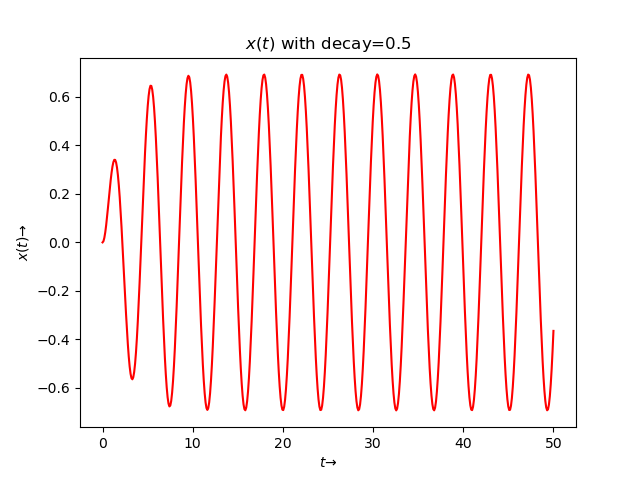
\includegraphics[scale=0.4]{fig1_6.png}
\caption{System Response with Decay = 0.5}
\label{fig:System Response with Decay = 0.5}
\end{figure}



\begin{figure}[h!]
\centering
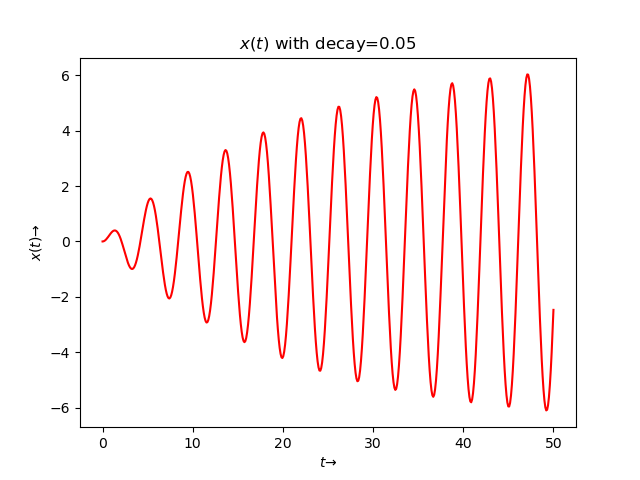
\includegraphics[scale=0.4]{fig2_6.png}
\caption{System Response with Decay = 0.05}
\label{fig:System Response with Decay = 0.05}
\end{figure}
\clearpage
We notice that the result are very similar except with a different amplitude. This is because the system takes longer to reach a steady state.

\section*{Question 3}
Considering the system with $f(t)$ input and $x(t)$ output.We now see what happens when we vary the frequency.We note the the amplitude is maximum at frequency = 1.5, which is the natural frequency of the given system
\begin{verbatim}
H = sp.lti([1],[1,0,2.25])
freq=np.linspace(1.4,1.6,5)
for w in freq:
	t = np.linspace(0,50,500)
	f = np.cos(w*t)*np.exp(-0.05*t)
	t,x,svec = sp.lsim(H,f,t)
	
	plt.figure(3)
	plt.plot(t,x,label='w = ' + str(w))
	plt.title("x(t) for different frequencies")
	plt.xlabel(r'$t\rightarrow$')
	plt.ylabel(r'$x(t)\rightarrow$')
	plt.legend(loc = 'upper left')  
	plt.show()
\end{verbatim}
\begin{figure}[h!]
\centering
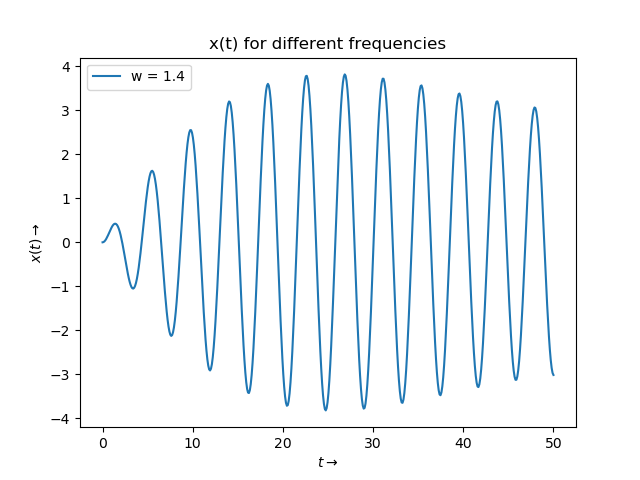
\includegraphics[scale=0.65]{fig3_6.png}
\caption{System Response with frequency = 1.4}
\label{fig:System Response with frequency = 1.4}
\end{figure}

\begin{figure}[h!]
\centering
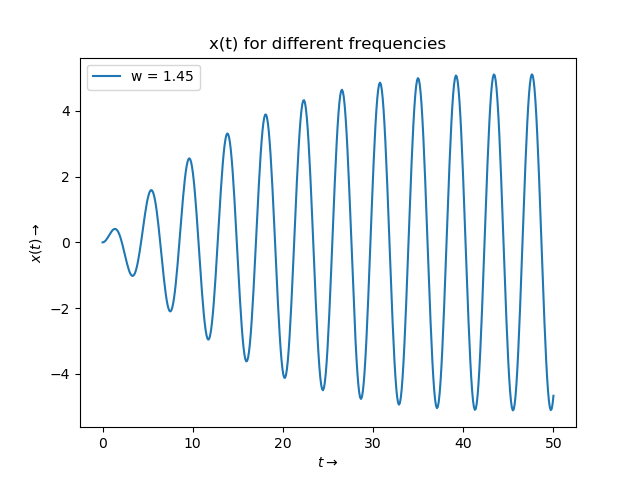
\includegraphics[scale=0.7]{fig4_6.png}
\caption{System Response with frequency = 1.45}
\label{fig:System Response with frequency = 1.45}
\end{figure}

\begin{figure}[h!]
\centering
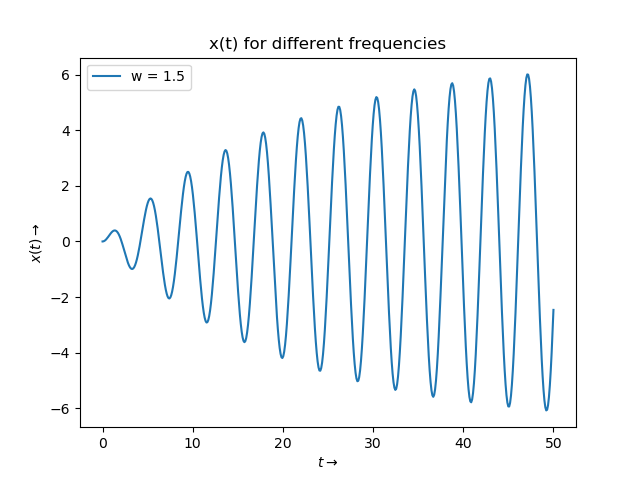
\includegraphics[scale=0.7]{fig5_6.png}
\caption{System Response with frequency = 1.5}
\label{fig:System Response with frequency = 1.5}
\end{figure}

\begin{figure}[h!]
\centering
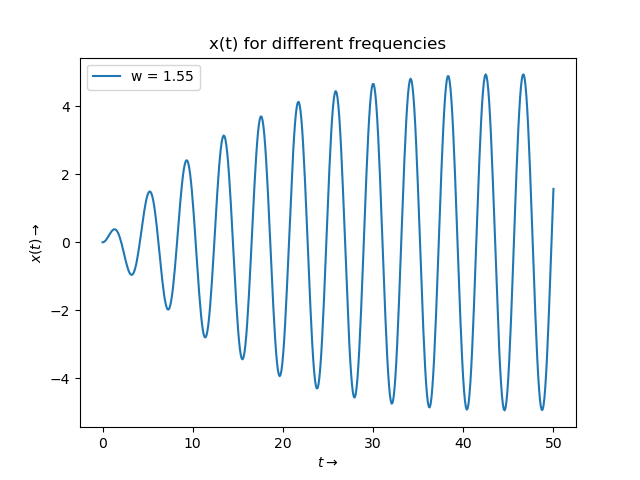
\includegraphics[scale=0.7]{fig6_6.png}
\caption{System Response with frequency = 1.55}
\label{fig:System Response with frequency = 1.55}
\end{figure}

\begin{figure}[h!]
\centering
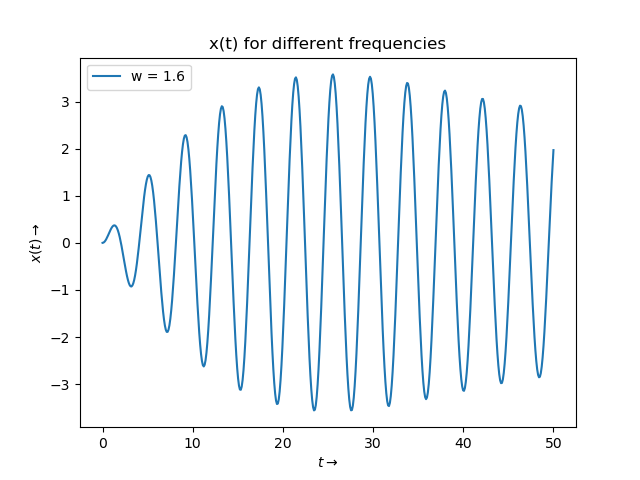
\includegraphics[scale=0.7]{fig7_6.png}
\caption{System Response with frequency = 1.6}
\label{fig:System Response with frequency = 1.6}
\end{figure}
\clearpage
\section*{Question 4}
We now consider a coupled Differential system
\begin{equation}
    \ddot x + (x-y) = 0
\end{equation}
and 
\begin{equation}
    \ddot y + 2(y-x) = 0
\end{equation}
with the initial conditions: $\dot x(0) =0,\dot y(0) =0,x(0) =1,y(0) =0$.
Taking Laplace Transform and solving for $X(s)$ and $Y(s)$, We get:
\begin{equation}
    X(s) = \frac{s^2+2}{s^3 + 3s}
\end{equation}
\begin{equation}
    Y(s) = \frac{2}{s^3 + 3s}
\end{equation}
\begin{verbatim}
#solve for X in coupling equation
t4 = np.linspace(0,20,500)
X4 = sp.lti([1,0,2],[1,0,3,0])
Y4 = sp.lti([2],[1,0,3,0])	
t4,x4 = sp.impulse(X4,None,t4)
t4,y4 = sp.impulse(Y4,None,t4)

plt.figure(4)   
plt.plot(t4, x4,'r')
plt.title(r"Time evolution of $x(t)$ for Coupled spring system")
plt.xlabel(r"$t \to $")
plt.ylabel(r"$x(t) \to $")
plt.show()

plt.figure(5)   
plt.plot(t4, y4,'r')
plt.title(r"Time evolution of $y(t)$ for Coupled spring system ")
plt.xlabel(r"$t \to $")
plt.ylabel(r"$y(t) \to $")
plt.show()
\end{verbatim}
We notice that the outputs of this system are 2 sinusoids which are out of phase.The amplitude of y is greater than that of x.
\begin{figure}[h!]
\centering
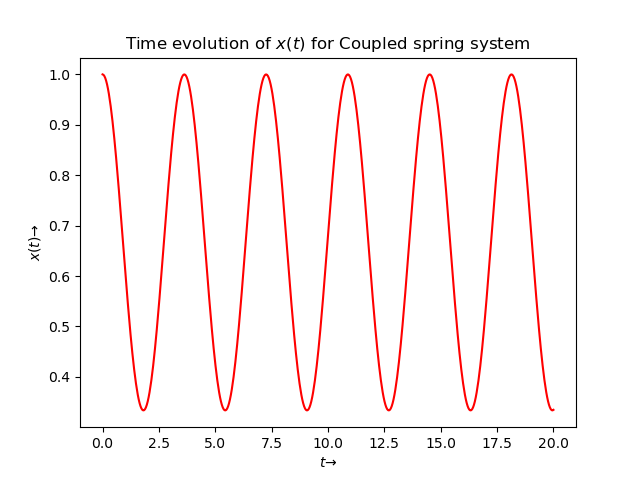
\includegraphics[scale=0.7]{fig8_6.png}
\caption{Coupled Oscillations}
\label{fig:Coupled Oscillations}
\end{figure}
\begin{figure}[h!]
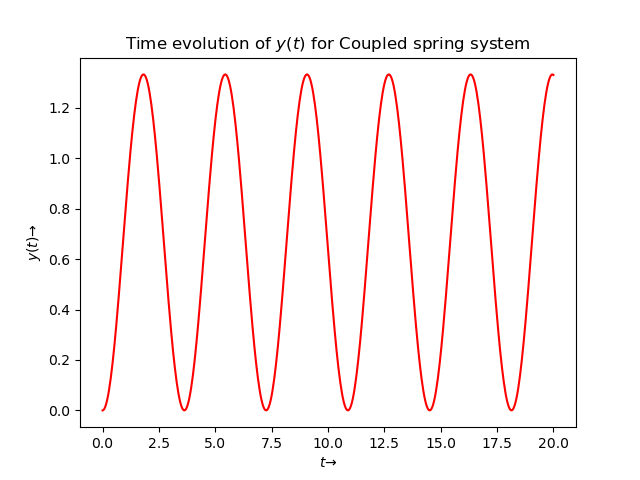
\includegraphics[scale=0.7]{fig9_6.png}
\caption{Coupled Oscillations }
\label{fig:Coupled Oscillations}
\end{figure}
\clearpage
\section*{Question 5}

Now we try to create the bode plots for the low pass filter defined in the question
\begin{verbatim}
def RLC_transfunc(R, C, L):
    Hnum = np.poly1d([1])
    Hden = np.poly1d([L*C, R*C, 1])
    Hs = sp.lti(Hnum, Hden)
    w, mag, phi = Hs.bode()
    return w, mag, phi, Hs

w, mag, phi, H = RLC_transfunc(100, 1e-6, 1e-6)

# plot Magnitude Response
plt.figure(6)
plt.semilogx(w, mag)
plt.title(r" Magnitude Response of $H(jw)$ of Series RLC network")
plt.xlabel(r"$ w \to $")
plt.ylabel(r"$ 20\log|H(jw)|  \to $")
plt.show()

# Plot of phase response
plt.figure(7)
plt.semilogx(w, phi, 'r', label="$Phase Response$")
plt.title(r"Phase response of the $H(jw)$ of Series RLC network")
plt.xlabel(r"$  w \to $")
plt.ylabel(r"$ \angle H(j\omega)$ $\to $")
plt.show()
\end{verbatim}

\begin{figure}[h!]
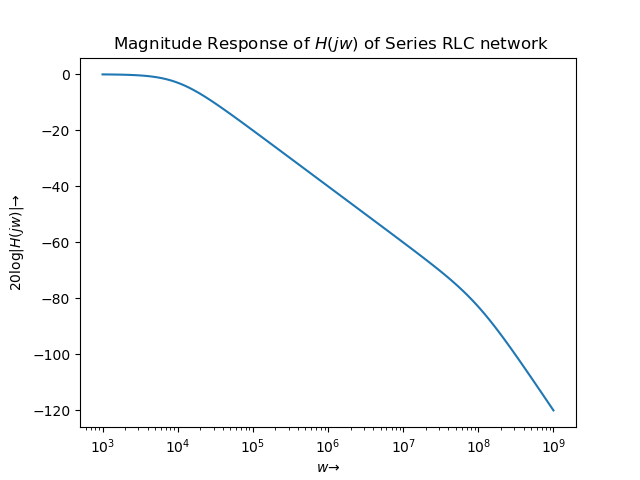
\includegraphics[scale=0.5]{fig10_6.png}
\centering
\caption{Magnitude Plot For RLC filter}
\label{Magnitude Plot For RLC filter}
\end{figure}
\begin{figure}[h!]
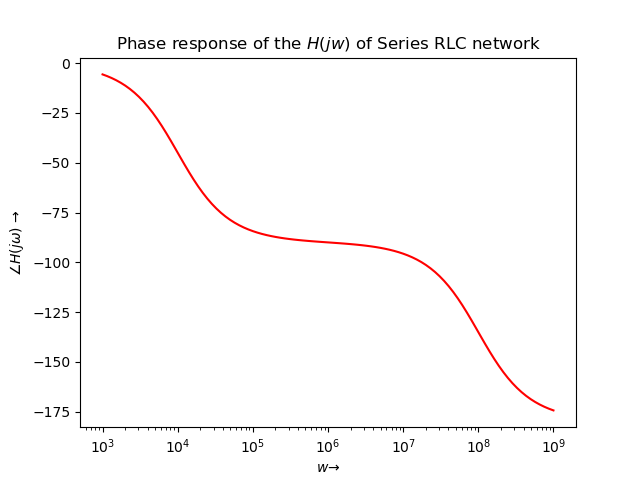
\includegraphics[scale=0.6]{fig11_6.png}
\centering
\caption{Phase Plot For RLC filter}
\label{Phase Plot For RLC filter}
\end{figure}


\section*{Question 6}
We now plot the response of the low pass filter to the input for different time variations:\newline
\begin{center}
$V_i(t) = (cos(10^3t) - cos(10^6t))u(t)$
\end{center}\newline
for $0<t<30\mu s$ and $0<t<30ms$


\begin{verbatim}
t = np.arange(0, 90*pow(10, -3), pow(10, -6))
vi = np.cos(t*pow(10, 3))-np.cos(t*pow(10, 6))
t, vo, svec = sp.lsim(H, vi, t)

# plot of Vo(t) for large time i.e at steady state
# Long term response
plt.figure(8)
plt.plot(t, vo, 'r')
plt.title(r"Output voltage $v_0(t)$ at Steady State")
plt.xlabel(r"$ t \to $")
plt.ylabel(r"$ y(t) \to $")
plt.show()

# Plot of Vo(t) for 0<t<30usec
plt.figure(9)
plt.plot(t, vo, 'r')
plt.title(r"Output voltage $v_0(t)$ for $0<t<30\mu sec$")
plt.xlim(0, 30*(10**(-6)))
plt.ylim(-1e-5, 0.3)
plt.xlabel(r"$ t \to $")
plt.ylabel(r"$ v_0(t) \to $")
plt.show()
\end{verbatim}



\begin{figure}[h!]
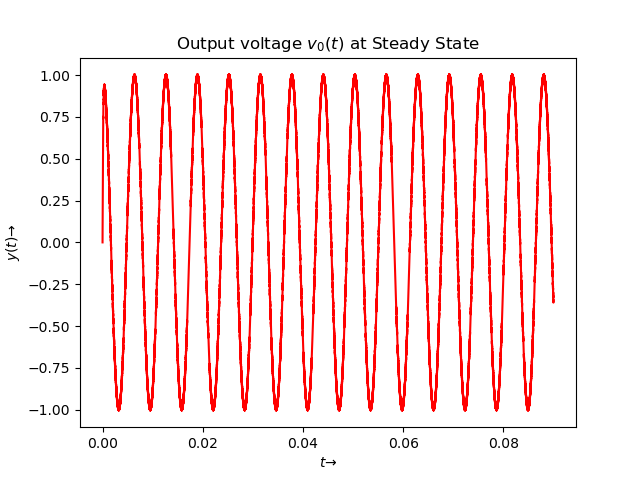
\includegraphics[scale=0.5]{fig12_6.png}
\centering
\caption{System response for t<30us}
\label{fig:Coupled Oscillations}
\end{figure}
\begin{figure}[h!]
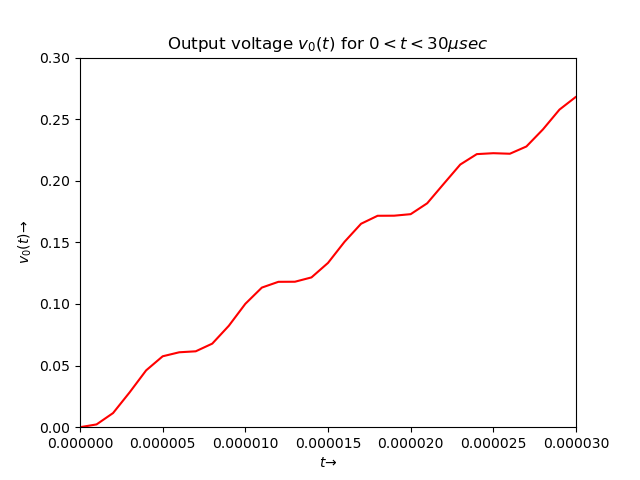
\includegraphics[scale=0.5]{fig13_6.png}
\centering
\caption{System response for t<30ms}
\label{fig:Coupled Oscillations}
\end{figure}
\clearpage

\section*{Conclusion}
In this assignment, we have used scipy's signal processing library to analyze some LTI systems. In the first system we noticed that oscillation amplitude settles to afixed value in both cases but it takes longer to settle if the decay is less.And we also observed that amplitude is maximum when input frequency is equal to natural frequency.

\end{document}
